In the following, seven applications are presented to illustrate the versatility of Bioptim and to give a practical overview on how to use its main features.
The performances and the Github links of each OCP are summarized in Tab.~\ref{tab:Perfs_and_detailed_implementations_of_each_example}.


\subsection{Muscle activation driven pointing task}
%
\begin{figure}[t!]
\centering
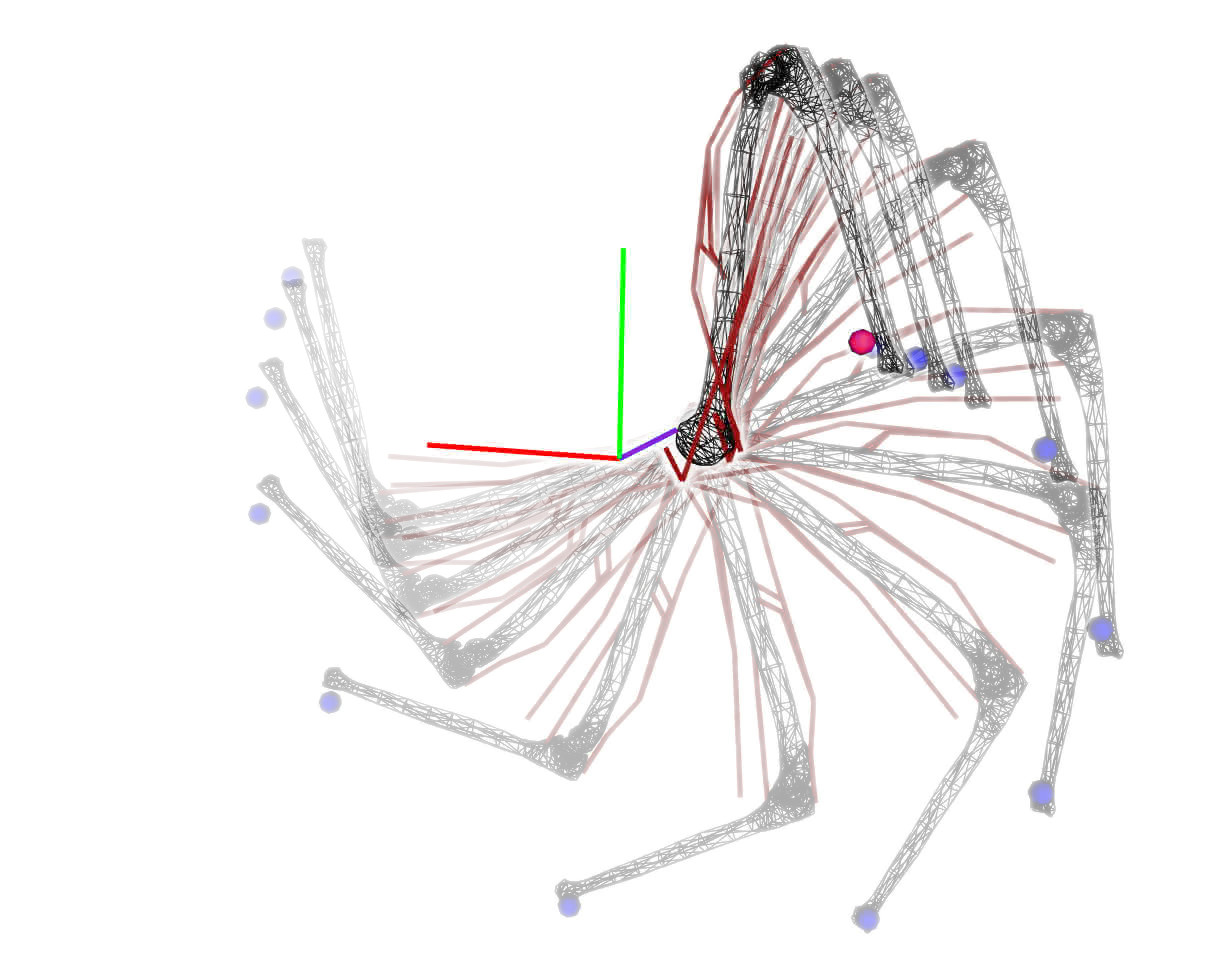
\includegraphics[width=\columnwidth]{figures/activation_pointing.jpeg}\\
\caption{Snapshots of an optimized activation-driven pointing task with \acados. The arm starts facing upwards in left hand part of the picture and ends facing downwards in the right hand part. The marker fized on the Ulna is depicted in blue and the scene-fixed target marker is depicted in red. Red lines show the lines of actions of the muscles.}
\label{fig:snapshots_activation_driven_pointing}
\end{figure}
\begin{figure*}[t!]
\centering
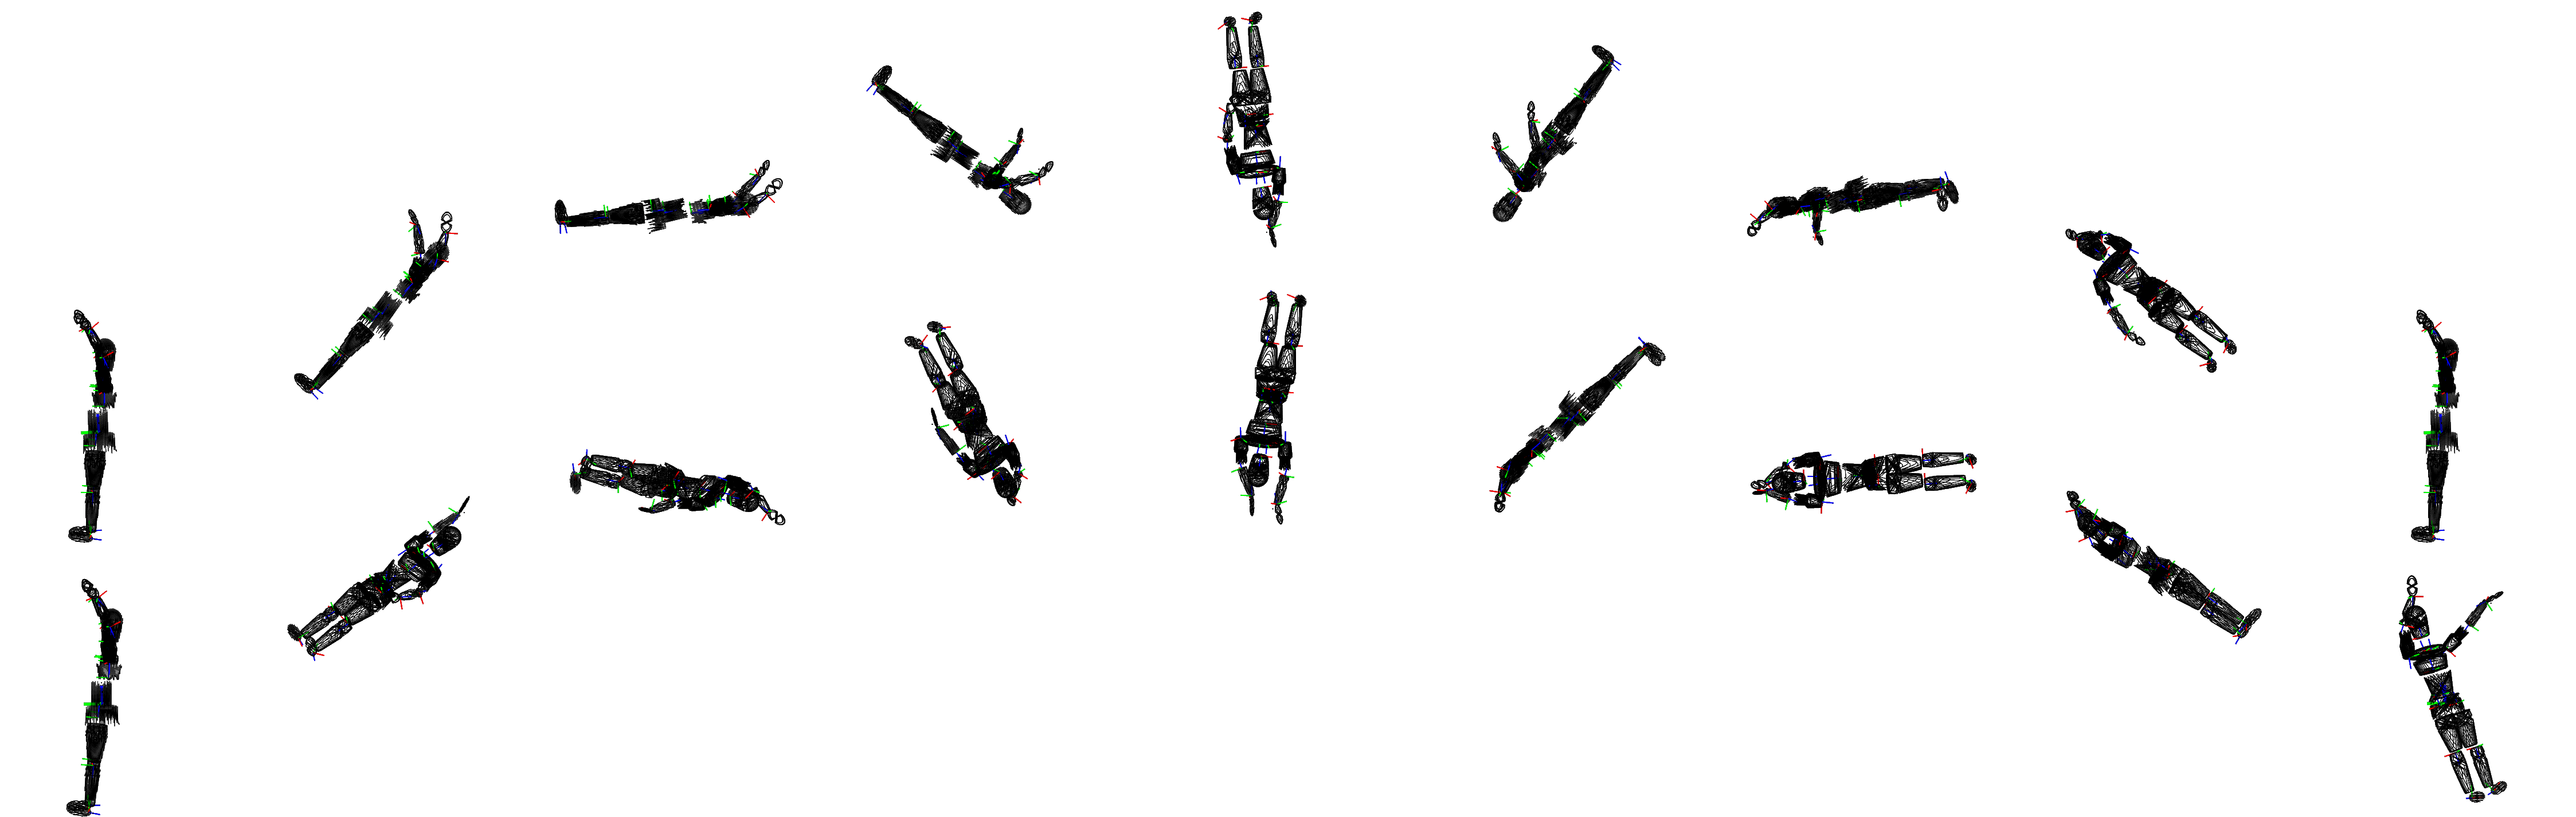
\includegraphics[width=\textwidth]{figures/Both_Bioptim_MaxVrille.png}
\caption{Snapshots of maximally twisting somersaults driven by shoulder torque actuators and a free base whose rotation is either expressed by Euler angles (top) or by quaternions (bottom).}
\label{fig:snapshots_quaternion_base_twisting_somersault}
\end{figure*}
%
In this first example, the goal was to achieve a muscle activation driven pointing task using a 2-DoF arm model with 6 muscle elements. 
In addition to muscle-induced torques, pure joint torques were added to compensate for the model weaknesses.
The main term (highest weight) of the objective function (Eq.~\ref{eq:cost_pointing}) is a Mayer objective, corresponding to the pointing tasks at the final node, to superimpose two markers, the first one, $\mathbf{m_u}$, fixed in the Ulna system of coordinates and the second one, $\mathbf{m^*_s}$, fixed in the scene.
The three Lagrange terms  were added for control regularization (muscle activation $\bf{a}$ and joint torques $\boldsymbol{\tau}$) and for state ($\bf{x}$) regularization:
\[
\begin{aligned}
	\mathcal{C} = 	&~\omega_1~\underbrace{\|\mathbf{m_u}(T)-\mathbf{m^*_s}\|^2}_{\mathtt{TRACK\_MARKERS}}~\\
	&\int_{t=0}^T\underbrace{\|\bf{a}\|^2}_{\mathtt{MIN\_ACTIVATION}}~
	+\underbrace{\|\boldsymbol\tau\|^2}_{\mathtt{MIN\_TORQUE}}~
	+\underbrace{\|\bf{x}\|^2}_{\mathtt{MIN\_STATE}}~ dt,
\end{aligned}
\addtag
\label{eq:cost_pointing}
\]

\noindent where T is the duration of the motion, and $\omega_1=1e5$.
The movement lasted for 2~seconds and was discretized using 50~shooting nodes with a 5-steps RK4 integration in-between.
The problem was solved using \ipopt (with exact Hessian computations) and \acados (with a Gauss-Newton approximation of the Hessian) resulting in two very close solutions.
\acados was about 50 times faster than \ipopt and was better at enforcing the continuity constraints (as shown by the single shooting error in Tab.~\ref{tab:Perfs_and_detailed_implementations_of_each_example}).
\ipopt however ended up with a smaller optimized objective (20.8 \textit{vs} 23.2), leading to a more optimal solution than \acados. 
Superimposed snapshots of the optimal motion found with \acados are displayed in Fig.~\ref{fig:snapshots_activation_driven_pointing}.
It is worth mentioning that for the purpose of this illustration, no constraint was given on the shoulder range of motion to ensure physiological muscle trajectories. 










\subsection{Quaternion base twisting somersault}
The goal was to maximize the twist rotation ($\phi$) in a backward somersault.
The model is composed of a 6-DoF root segment and two 1-DoF torque actuated arms.
The OCP was solved for two models.
First, rotations of the root segment were expressed as Euler angles.
They were expressed as a quaternion for the second model.
The objective functions were written as follow:

\begin{eqnarray}\label{eq:ocp_Trampo}
\mathcal{J} = -\underbrace{\int_0^T \dot{\phi}~dt}_{MINIMIZE\_TWIST}  +~\omega_1 \underbrace{\int_0^T \sum_{i=1}^{2}~\tau_{i}^2~dt}_{MINIMIZE\_ TORQUE},
\end{eqnarray}
with $\omega_1 = 1\times 10^{-6}$, T the duration of the movement and $\tau_{i}$ the torque control of the $i^{th}$ arm DoF.
The first term of the objective function (Eq.~\ref{eq:ocp_Trampo}) corresponds to maximizing the twist velocity and the second term is for control regularization.


The movement lasted for approximately 1 second and was discretized in 100 shooting nodes.
The solutions for both models were similar (Fig.~\ref{snapshots_quaternion_base_twisting_somersault}) highlighting the equivalence of the two rotation representations.
Euler angles have the advantage to be easily interpretable, but they suffer from the loss of a DoF at the gimbal lock.
The use of quaternion representation is advantageous for numerical stability when a joint is free to rotate on a wide three-dimensional range for motion.


\begin{figure*}[t!]
\centering
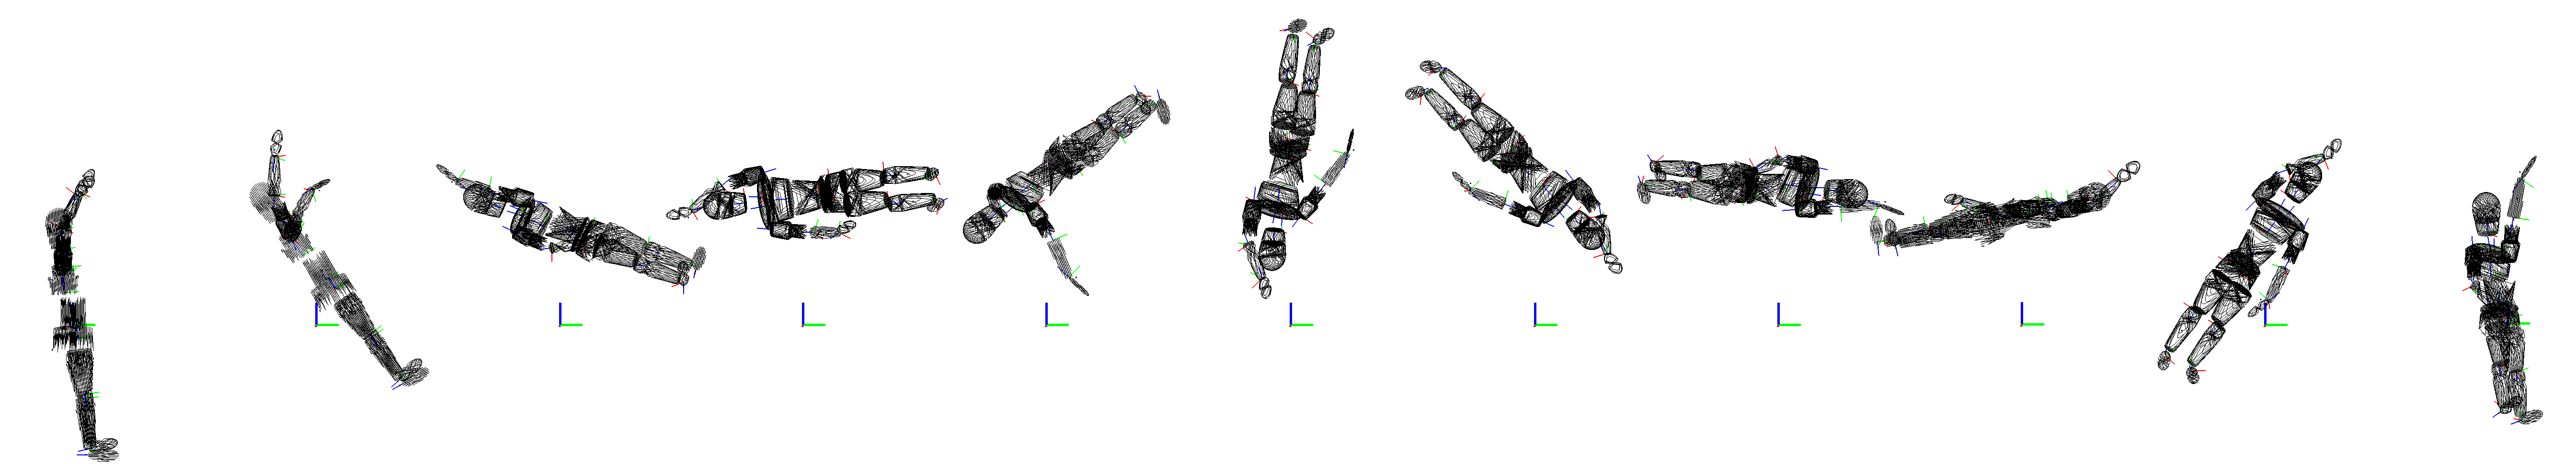
\includegraphics[width=\textwidth]{figures/Euler_Bioptim_MaxVrille_2.png}\\
\vspace*{0.5em}
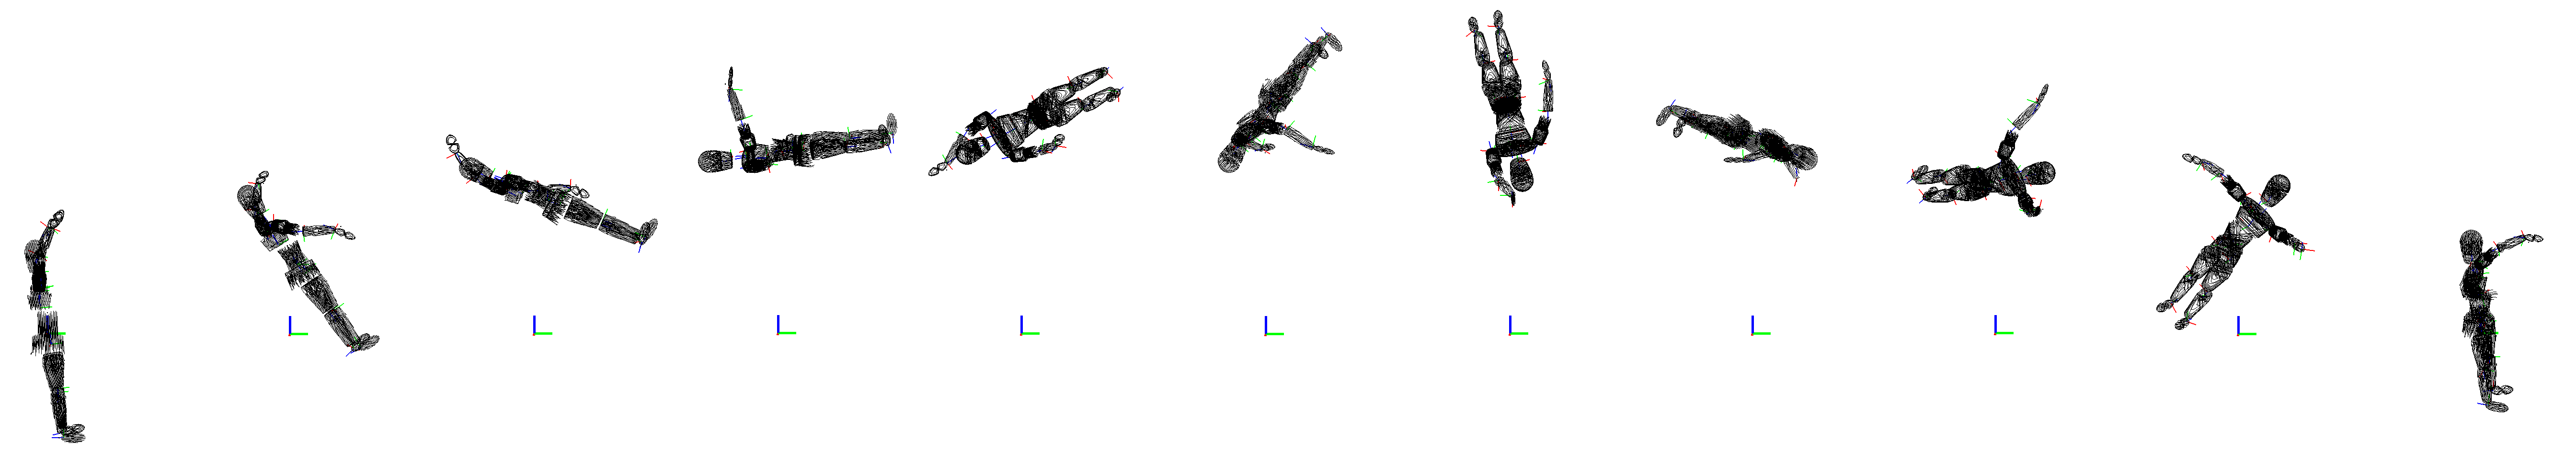
\includegraphics[width=\textwidth]{figures/Quat_Bioptim_MaxVrille_2.png}
\caption{Snapshots of a maximally twisting somersault driven by shoulder torque actuators and a free base expressed by Euler angles (top) or quaternions (bottom).}
\label{fig:snapshots_quaternion_base_twisting_somersault}
\end{figure*}


% \begin{table}[h!]
% \caption{\small Objective terms of quaternion base maximally twisting somersault}
% \label{tab:Quaternion_base_twisting_somersault}
% \centering
% \begin{tabular}{c c c c}
% \toprule 
% & Type & Function & Weight \\ 
% \midrule
% $\#1$ & Lagrange & MINIMIZE\_TWIST & $-1e1$ \\ 
% \midrule
% $\#2$ & Lagrange & MINIMIZE\_ TORQUE & $1e-6$ \\ 
% \bottomrule
% \end{tabular}
% \end{table}















%
\begin{table*}[t!]
\caption{\small Overview of computational results for the different OCPs cases and links to detailed implementations. $^\star$ stands for free time OCP, otherwise it is fixed.}
\label{tab:Perfs_and_detailed_implementations_of_each_example}
\centering
\begin{tabular}{c l rl rl rl}
\cmidrule[\heavyrulewidth](lr){2-8}
& & \multicolumn{2}{l}{Activation-driven pointing} & \multicolumn{2}{l}{Ex\# 2} & \multicolumn{2}{l}{Ex\# 3} \\
\cmidrule[\heavyrulewidth](lr){3-4}
\cmidrule[\heavyrulewidth](lr){5-6}
\cmidrule[\heavyrulewidth](lr){7-8}

\mymultirow{4}{Setup} & \# states $\xt$            & \multicolumn{2}{c}{2}  & --    & --     & --    & --\\
                      & \# control $\ut$           & \multicolumn{2}{c}{8}  & --    & --     & --    & --\\
                      & \# shooting nodes          & \multicolumn{2}{c}{51} & --    & --     & --    & --\\
                      & OCP duration (s)           & \multicolumn{2}{c}{2}  & --    & --     & --    & --\\
                      &                            & IPOpt  & ACADOS        & IPOpt & ACADOS & IPOpt & ACADOS\\
\mymultirow{3}{Solve} & \# NLP iterations          & 27     & 21            & --    & --     & --    & --\\
                      & Optimized cost             & 6959.3 & 427.5         & --    & --     & --    & --\\
                      & Time to convergence (s)    & 9.9    & 0.19          & --    & --     & --    & --\\
%Example & Link & IPOPT & ACADOS \\ 
%\midrule
%Muscle activation driven pointing task & \href{https://github.com/pyomeca/BiorbdOptim/blob/master/examples/muscle_driven_ocp/static_arm.py}{$\star$} & $10.10$ & $0.2018$  \\ 
%\midrule
%$\bullet$ & $\bullet$ & $\bullet$ & $\bullet$ \\ 
\cmidrule[\heavyrulewidth](lr){2-8}
\end{tabular}
\end{table*}
%







